%  !TeX  root  =  user_guide.tex

\section{Plugin grafo strade}\label{sec:roadgraph}

% when the revision of a section has been finalized, 
% comment out the following line:
% \updatedisclaimer


\toolbtntwo{plugin}{Plugin grafo strade} è un plugin scritto in C++ che calcola il percorso minimo 
tra punti su una polilinea e traccia tale percorso sul grafo delle strade.

\textbf{Caratteristiche principali}:

\begin{itemize}
\item Calcola il percorso, la sua lunghezza ed il tempo di percorrenza
\item Ottimizza la lunghezza ed il tempo di percorrenza
\item Esporta il percorso in un layer vettoriale
\item Evidenzia la direzione delle strade (tale funzionalità è lenta e dovrebbe essere usata solo in fase di test)
\end{itemize}

Come layer di strade è possibile usare un layer vettoriale di polilinee in uno dei formati supportati da QGIS.
Due linee con un punto in comune vengono considerate connesse. Si noti che è richiesto di impostare il SR del 
progetto sul SR del layer qualora si intenda modificare quest'ultimo: il ricalcolo delle coordinate in differenti 
SR introduce degli errori che inficiano la qualità dei dati, anche se si opera con lo snap attivato. 

\textbf{Nella tabella degli attributi del layer si possono usare i seguenti campi}:

\begin{itemize}
\item Velocità su sezione di strada — numerico
\item Direzione — testo (avanti, inversa, a doppio senso)
\end{itemize}

Se alcuni campi non hanno valori, o non esistono, vengono utilizzati dei valori predefiniti.

\minisec{Utilizzo del plugin}

Una volta caricato il plugin, impostarne le opzioni nella finestra di dialogo \dialog{Impostazioni del plugin grafo strade} 
(\mainmenuopt{Plugins} \arrow \dropmenuopt{Road Graph (grafo strade)}). 

\begin{figure}[ht]
    \centering
    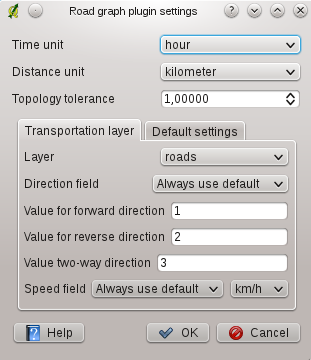
\includegraphics[clip=true, width=10cm]{roadgraph_settings}
    \caption{Impostazioni del plugin grafo strade \nixcaption}\label{fig:roadgraphsettings}
\end{figure}

Selezionare un punto di partenza ed un punto di arrivo sul grafo delle strade e cliccare su \button{Calcola}.

\begin{figure}[ht]
    \centering
    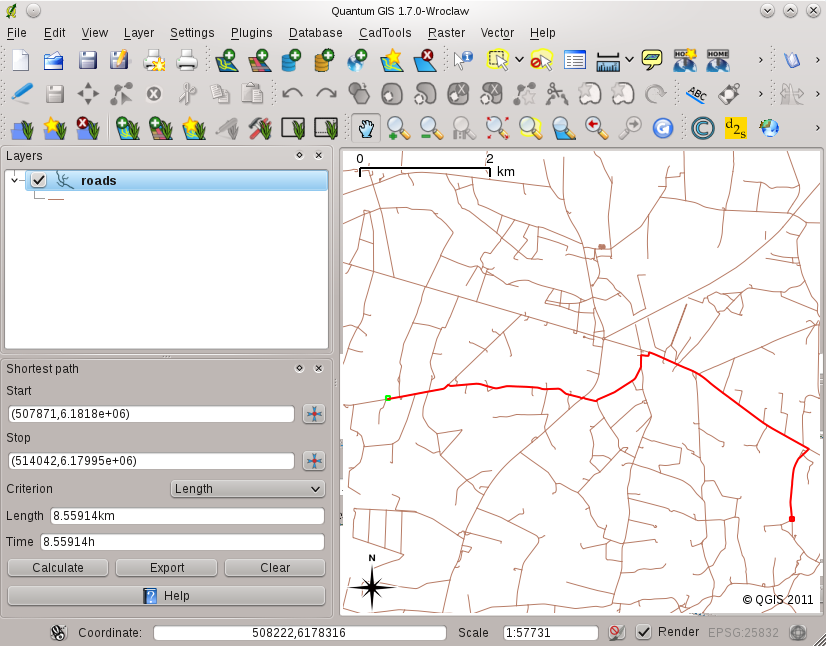
\includegraphics[clip=true, width=12cm]{roadgraph_sample}
    \caption{Plugin grafo strade \nixcaption}\label{fig:roadgraphsample}
\end{figure}

\FloatBarrier